% Created by tikzDevice version 0.12.3.1 on 2021-05-13 15:20:03
% !TEX encoding = UTF-8 Unicode
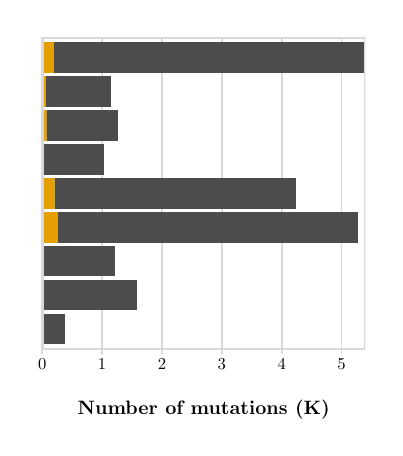
\begin{tikzpicture}[x=1pt,y=1pt]
\definecolor{fillColor}{RGB}{255,255,255}
\path[use as bounding box,fill=fillColor,fill opacity=0.00] (0,0) rectangle (125.50,144.54);
\begin{scope}
\path[clip] (  5.25, 28.30) rectangle (122.00,141.04);
\definecolor{drawColor}{gray}{0.85}

\path[draw=drawColor,line width= 0.6pt,line join=round] (  5.25, 28.30) --
	(  5.25,141.04);

\path[draw=drawColor,line width= 0.6pt,line join=round] ( 26.88, 28.30) --
	( 26.88,141.04);

\path[draw=drawColor,line width= 0.6pt,line join=round] ( 48.52, 28.30) --
	( 48.52,141.04);

\path[draw=drawColor,line width= 0.6pt,line join=round] ( 70.15, 28.30) --
	( 70.15,141.04);

\path[draw=drawColor,line width= 0.6pt,line join=round] ( 91.78, 28.30) --
	( 91.78,141.04);

\path[draw=drawColor,line width= 0.6pt,line join=round] (113.41, 28.30) --
	(113.41,141.04);
\definecolor{fillColor}{gray}{0.30}

\path[fill=fillColor] (  9.55,128.17) rectangle (122.00,139.20);
\definecolor{fillColor}{RGB}{230,159,0}

\path[fill=fillColor] (  5.25,128.17) rectangle (  9.55,139.20);
\definecolor{fillColor}{gray}{0.30}

\path[fill=fillColor] (  6.48,115.92) rectangle ( 29.95,126.95);
\definecolor{fillColor}{RGB}{230,159,0}

\path[fill=fillColor] (  5.25,115.92) rectangle (  6.48,126.95);
\definecolor{fillColor}{gray}{0.30}

\path[fill=fillColor] (  6.87,103.67) rectangle ( 32.66,114.69);
\definecolor{fillColor}{RGB}{230,159,0}

\path[fill=fillColor] (  5.25,103.67) rectangle (  6.87,114.69);
\definecolor{fillColor}{gray}{0.30}

\path[fill=fillColor] (  5.25, 91.41) rectangle ( 27.44,102.44);

\path[fill=fillColor] (  9.79, 79.16) rectangle ( 96.78, 90.19);
\definecolor{fillColor}{RGB}{230,159,0}

\path[fill=fillColor] (  5.25, 79.16) rectangle (  9.79, 90.19);
\definecolor{fillColor}{gray}{0.30}

\path[fill=fillColor] ( 10.96, 66.90) rectangle (119.47, 77.93);
\definecolor{fillColor}{RGB}{230,159,0}

\path[fill=fillColor] (  5.25, 66.90) rectangle ( 10.96, 77.93);
\definecolor{fillColor}{gray}{0.30}

\path[fill=fillColor] (  5.94, 54.65) rectangle ( 31.64, 65.68);
\definecolor{fillColor}{RGB}{230,159,0}

\path[fill=fillColor] (  5.25, 54.65) rectangle (  5.94, 65.68);
\definecolor{fillColor}{gray}{0.30}

\path[fill=fillColor] (  5.25, 42.40) rectangle ( 39.36, 53.42);

\path[fill=fillColor] (  5.47, 30.14) rectangle ( 13.32, 41.17);
\definecolor{fillColor}{RGB}{230,159,0}

\path[fill=fillColor] (  5.25, 30.14) rectangle (  5.47, 41.17);

\path[draw=drawColor,line width= 1.1pt,line join=round,line cap=round] (  5.25, 28.30) rectangle (122.00,141.04);
\end{scope}
\begin{scope}
\path[clip] (  0.00,  0.00) rectangle (125.50,144.54);
\definecolor{drawColor}{gray}{0.85}

\path[draw=drawColor,line width= 0.6pt,line join=round,line cap=rect] (  5.25, 28.30) --
	(  5.25,141.04);
\end{scope}
\begin{scope}
\path[clip] (  0.00,  0.00) rectangle (125.50,144.54);
\definecolor{drawColor}{gray}{0.85}

\path[draw=drawColor,line width= 0.6pt,line join=round] (  5.25, 26.55) --
	(  5.25, 28.30);

\path[draw=drawColor,line width= 0.6pt,line join=round] ( 26.88, 26.55) --
	( 26.88, 28.30);

\path[draw=drawColor,line width= 0.6pt,line join=round] ( 48.52, 26.55) --
	( 48.52, 28.30);

\path[draw=drawColor,line width= 0.6pt,line join=round] ( 70.15, 26.55) --
	( 70.15, 28.30);

\path[draw=drawColor,line width= 0.6pt,line join=round] ( 91.78, 26.55) --
	( 91.78, 28.30);

\path[draw=drawColor,line width= 0.6pt,line join=round] (113.41, 26.55) --
	(113.41, 28.30);
\end{scope}
\begin{scope}
\path[clip] (  0.00,  0.00) rectangle (125.50,144.54);
\definecolor{drawColor}{RGB}{0,0,0}

\node[text=drawColor,anchor=base,inner sep=0pt, outer sep=0pt, scale=  0.60] at (  5.25, 20.92) {0};

\node[text=drawColor,anchor=base,inner sep=0pt, outer sep=0pt, scale=  0.60] at ( 26.88, 20.92) {1};

\node[text=drawColor,anchor=base,inner sep=0pt, outer sep=0pt, scale=  0.60] at ( 48.52, 20.92) {2};

\node[text=drawColor,anchor=base,inner sep=0pt, outer sep=0pt, scale=  0.60] at ( 70.15, 20.92) {3};

\node[text=drawColor,anchor=base,inner sep=0pt, outer sep=0pt, scale=  0.60] at ( 91.78, 20.92) {4};

\node[text=drawColor,anchor=base,inner sep=0pt, outer sep=0pt, scale=  0.60] at (113.41, 20.92) {5};
\end{scope}
\begin{scope}
\path[clip] (  0.00,  0.00) rectangle (125.50,144.54);
\definecolor{drawColor}{RGB}{0,0,0}

\node[text=drawColor,anchor=base,inner sep=0pt, outer sep=0pt, scale=  0.70] at ( 63.63,  4.86) {\bfseries Number of mutations (K)};
\end{scope}
\end{tikzpicture}
